% \documentclass[12pt,a4j]{jsarticle}
\documentclass[12pt,a4paper]{article}
\usepackage[a4paper, margin=0.8in]{geometry}
\usepackage[ipaex]{pxchfon}
\usepackage[dvipdfmx]{graphicx}
\usepackage[utf8]{inputenc}
\usepackage[english]{babel}
\usepackage{multirow}
\usepackage{times}
\usepackage{amsmath}
\usepackage{amssymb}
\usepackage{amsfonts}
\usepackage{comment}
\usepackage{enumitem}
\usepackage{natbib}
\usepackage{hyperref}

\begin{document}
\pagenumbering{roman}

% title
\begin{titlepage}
    \title{\textbf{{\Large 工学院情報通信系情報通信コース 修士論文\\Master Thesis}}}
    \author{}
    \date{}
    \maketitle
    \thispagestyle{empty}
    \begin{center}
        \vspace{1.5cm}
        \textbf{{\Large Hogehoge Title}}
            
        \vspace{4cm}
        \author{\textbf{{\large{Fistname Lastname}}}}

        \vspace{1.5cm}
        Supervisor: Manabu Okumura\\
        Institute of Innovative Research\\
        Tokyo Institute of Technology
        \vfill
            
        A thesis presented for the degree of\\
        Master of Engineering
        \vspace{0.8cm}
     
        
\includegraphics[width=0.08\textwidth]{figures/titech-logo.png}
        
        School of Engineering\\
        Department of Information and Communications Engineering\\
        Tokyo Institute of Technology\\
        \vspace{0.8cm}
        Submitted on \date{\today}
   \end{center}
\end{titlepage}

\clearpage

\newgeometry{left=4cm}
\newenvironment{xlist}{%
  \begin{list}{}{%
    \setlength{\labelwidth}{0em}
    \setlength{\labelsep}{0em}
    \setlength{\leftmargin}{\labelwidth}
    \addtolength{\leftmargin}{\labelsep}
    \setlength{\rightmargin}{0pt}
    \setlength{\parsep}{0ex plus 0.2ex minus 0.1ex}
    \setlength{\itemsep}{0.1ex plus 0.2ex}
  }
}
{\end{list}}
\thispagestyle{empty}
    \begin{center}
        \vspace*{6cm}
        A Master Thesis\\
        Submitted to School of Engineering,\\
        Department of Information and Communications Engineering,\\
        Tokyo Institute of Technology,\\
        in partial fulfillment of the requirements for the degree of\\
        Master of Engineering

        \vspace{1cm}
        Firstname Lastname
   \end{center}

\vspace{1cm}
\begin{flushleft}
    Thesis Committee:
    \begin{xlist}
        \item Manabu Okumura (Supervisor)\\(Professor, Tokyo Institute of Technology)
        \item Manabu Okumura\\(Professor, Tokyo Institute of Technology)
        \item Manabu Okumura\\(Professor, Tokyo Institute of Technology)
    \end{xlist}
\end{flushleft}

% do not remove
\restoregeometry
\clearpage

% abstract
% Large abstract header command
\renewcommand{\abstractname}{\large Abstract}
% Keywords command
\providecommand{\keywords}[1]
{
  \small	
  \textbf{\textit{Keywords---}} #1
}
\thispagestyle{empty}

\begin{center}
    \vspace*{1cm}
    
    \textbf{\Large Hogehoge Title}
    \vspace{1.5cm}
    
    {\large Fastname  Lastname}
    \vspace{1.5cm}    
\end{center}
 
\begin{abstract}
こんにちは Hogehoge, こんにちは Hogehoge, こんにちは Hogehoge, こんにちは Hogehoge, こんにちは Hogehoge, こんにちは Hogehoge, こんにちは Hogehoge, こんにちは Hogehoge, こんにちは Hogehoge, こんにちは Hogehoge, こんにちは Hogehoge, こんにちは Hogehoge, こんにちは Hogehoge, こんにちは Hogehoge, こんにちは Hogehoge, こんにちは Hogehoge, こんにちは Hogehoge, こんにちは Hogehoge, こんにちは Hogehoge, 
\end{abstract}

\keywords{Hogehoge keyword, Fugafuga keyword}

\clearpage

% acknowledgement
\addcontentsline{toc}{section}{Acknowledgments}
\vspace*{0.5cm}
\section*{\LARGE Acknowledgments}
\vspace{1cm}

Thank you. ありがとうございます。


\clearpage

% TOC
\tableofcontents
\clearpage

% figures
\addcontentsline{toc}{section}{\listfigurename}
\listoffigures
\cleardoublepage

% figures
\addcontentsline{toc}{section}{\tablename}
\listoftables
\cleardoublepage

% Set numbering for TOC
\pagenumbering{arabic}

% introduction

\section{Introduction}
Introduction Figure~\ref{fig:ex-fig}. Hoge \cite{devlin-etal-2019-bert}. Table~\ref{tab:ex-tab}.

\begin{figure}[h]
    \centering
    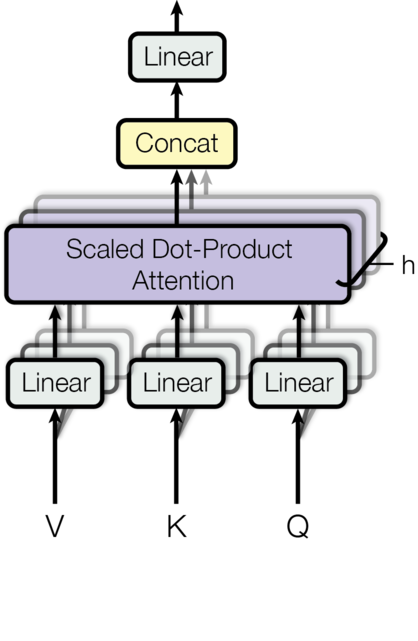
\includegraphics{figures/fig-vkq.png}
    \caption{Example figure.}
    \label{fig:ex-fig}
\end{figure}

\begin{table}[h]
    \centering
    \begin{tabular}{||c c c c||} 
        \hline
        Col1 & Col2 & Col2 & Col3 \\ [0.5ex] 
        \hline\hline
        1 & 6 & 87837 & 787 \\ 
        2 & 7 & 78 & 5415 \\
        3 & 545 & 778 & 7507 \\
        4 & 545 & 18744 & 7560 \\
        5 & 88 & 788 & 6344 \\ [1ex] 
        \hline
    \end{tabular}
    \caption{Example table.}
    \label{tab:ex-tab}
\end{table}
\clearpage

% related work
\section{Related Work}
\subsection{hoge}
\subsubsection{hogehoge}
\subsection{fuga}
\subsubsection{fugafuga}
\clearpage

% methodology
\section{Methodology}
\subsection{hoge}
    Equation~\ref{eq:ex-eq}.
    \begin{equation}
        \begin{split}
            y &= 2 + 2 \\
            &= 4.
        \end{split}
        \label{eq:ex-eq}
    \end{equation}
\subsubsection{hogehoge}
\subsection{fuga}
\subsubsection{fugafuga}
\clearpage

% experiments
\section{Experiments}
\subsection{hoge}
\subsubsection{hogehoge}
\subsection{fuga}
\subsubsection{fugafuga}
\clearpage

% results
\section{Results}
\subsection{hoge}
\subsubsection{hogehoge}
\subsection{fuga}
\subsubsection{fugafuga}
\clearpage

% experiments
\section{Conclusion}
Conclusion
\clearpage

% reference
\addcontentsline{toc}{section}{References}
\clearpage

% bib
\bibliographystyle{plainnat}
\bibliography{bib/anthology,bib/extra_ref}


\end{document}

